\documentclass{beamer}
\usepackage[english,russian]{babel}
\usepackage[utf8]{inputenc}
\usepackage[T1]{fontenc}
\usepackage{graphicx}
\usepackage{ulem}

\mode<presentation>
{
  \usetheme{Warsaw}
  \useoutertheme{miniframes}
  \setbeamercovered{transparent}
}

\begin{document}

\title{Очереди сообщений в распределённых системах}
\author{Максим 'max\_posedon' Мельников}
\institute{Linux Mobile hobbyist\\World of Tanks developer}
\date{\today}
\frame{\titlepage}

\frame{
    \frametitle{План}
    \tableofcontents
}

\section{Обзор различных MQ}
\frame{
    \frametitle{Очереди сообщений}
    \begin{block}{Что это такое?}
    Это архитектура и ПО промежуточного уровня, которое занимается сбором, хранением 
    и маршрутизацией (распределением) сообщений между компонентами. 
    \end{block}

    \begin{block}{Зачем?}
    Организация очереди сообщений помогает раз-балансировать нагрузку между различными узлами сети, 
    избавиться от единой точки отказа (SPOF),
    выполнять бизнес-логику приложения асинхронно, 
    повысить скорость ответа системы и многое другое.
    \end{block}
}

\frame{
    \frametitle{Apache ActiveMQ}
    \begin{itemize}
    \item Реализован на Java
    \item Полностью реализует Java Message Service 1.1 (JMS)
    \item "Enterprise Features": кластеризация, журнал операций, ...
    \end{itemize}
}

\frame{
    \frametitle{ZeroMQ}
    \begin{itemize}
    \item Реализован на C++
    \item Работает без сервера
    \item Низкоуровневое API
    \end{itemize}
}

\frame{
    \frametitle{PgQ}
    \begin{itemize}
    \item Реализован на C/SQL как расширение к PostgreSQL
    \item Тесная интеграция с базой данных (транзакции)
    \item Skype
    \end{itemize}
}

\frame{
    \frametitle{AMQP}
    \begin{block}{AMQP}
    Advanced Message Queueing Protocol   
    \end{block}

    \begin{block}{Apache Qpid}
    \begin{itemize}
    \item Реализация на C++
    \item RedHat
    \end{itemize}
    \end{block}

    \begin{block}{RabbitMQ server}
    \begin{itemize}
    \item Реализация на Erlang
    \item VMWare
    \end{itemize}
    \end{block}
}

\section{Архитектура AMQP}
\frame{
    \frametitle{Используемая терминология}
    \begin{itemize}
    \item Брокер (broker)
    \item Сообщение (mesasage)
    \item Точка обмена (exchange)
    \item Очередь (queue)
    \end{itemize}
}

\frame{
    \frametitle{Hello World}
    \begin{figure}[htb]
    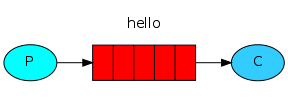
\includegraphics[width=\textheight]{hello.png}
    \end{figure}
}

\frame{
    \frametitle{Work queues}
    \begin{figure}[htb]
    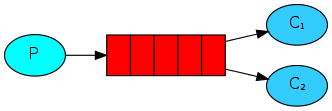
\includegraphics[width=\textwidth]{queues.png}
    \end{figure}
}

\frame{
    \frametitle{Publish/Subscribe}
    \begin{figure}[htb]
    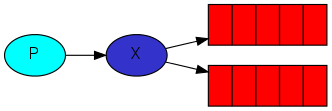
\includegraphics[width=\textwidth]{pubsub.png}
    \end{figure}
}

\frame{
    \frametitle{Routing}
    \begin{figure}[htb]
    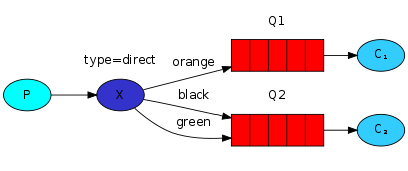
\includegraphics[width=\textwidth]{routing.png}
    \end{figure}
}

\frame{
    \frametitle{Topics}
    \begin{figure}[htb]
    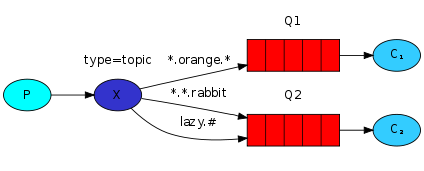
\includegraphics[width=\textwidth]{topics.png}
    \end{figure}
}

\frame{
    \frametitle{RPC}
    \begin{figure}[htb]
    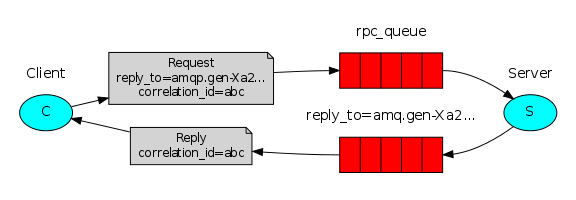
\includegraphics[width=\textwidth]{rpc.png}
    \end{figure}
}

\section{MQ в проекте World of Tanks}
\frame{
    \frametitle{Серверная инфраструктура игры}
    \begin{block}{Игровые сервера}
    \begin{itemize}
    \item LoginApp - аутентификация клиента
    \item DBMgr - управление базой данных
    \item MySQL (на самом деле несколько)
    \item BaseApp - управление аккаунтами (игра в ангар)
    \item СellApp - управление боями (игра в танчики)
    \end{itemize}
    \end{block}
    
    \begin{block}{WEB}
    \begin{itemize}
    \item SPA - сервис аутентификации
    \item Форумы
    \item Портал (worldoftanks.ru)
    \item Платёжная система
    \item ...
    \end{itemize}
    \end{block}
}

\frame{
    \frametitle{Экспорт данных из игрового сервера}
    \begin{itemize}
    \item Информация об аккаунте
    \item Информация о клане
    \item Информация о клановых/турнирных боях
    \end{itemize}
}

\frame{
    \frametitle{API игрового сервера}
    \begin{itemize}
    \item Создание аккаунта
    \item Начисление денег
    \item Управление кланом
    \item Создание клановых/турнирных боёв
    \end{itemize}
}

\frame{
    \frametitle{Асинхронные задачи на WEB проектах}
    \begin{block}{В обработке запроса участвуют сторонние ресурсы}
    \begin{itemize}
    \item Форумы
    \item Игровые сервера
    \item Социальные сети
    \item Внешние платёжные системы
    \end{itemize}
    \end{block}
}

\section{}
\frame{
    \frametitle{Вопросы}
    \begin{itemize}
    \item email/jabber(xmpp): m\_melnikau@wargaming.net
    \end{itemize}
}

\frame{
    \frametitle{Разыскиваются}
    \begin{itemize}
    \item Python-разработчики
    \item Linux-специалисты
    \item QA-специалисты
    \item Админ-ы
    \item Просто хорошие технические специалисты
    \end{itemize}
}

\end{document}

